\section{Interaction Model}
\label{sec:conceptual-interaction}

The Interaction Model is the third part of the XRM conceptual model. The Behavioural Model focused on defining the capabilities of Actors according to their roles.  Based on it, the Interaction Model aims to combine the different actions of users, the Target of these actions, and how one or more Actuators respond to this interaction.
Similar to the Behavioural Model, the Interaction Model defines primitives: the Interaction and the System Event.
In addition, it includes two sub-models distinguished by the level of abstraction. The one at a lower level aims to compose a more complex system starting from the primitives just defined: the Task. At a high level, on the other hand, the Activity is composed of a concatenation of Tasks and aims to provide a complete picture of the flow of the experience. 

\subsection*{Design of the Task: Low-Level Conceptualization}

In order to give a more exhaustive definition of the concept of Task, it is first required to explore two fundamental elements: Interaction and the System Event.

\subsubsection*{Interaction}

The \emph{Interaction} represents a process where a Human Actor performs actions on a Non-Human Actor, the Actuator, to complete a task. Each interaction is defined by the User’s Actions. 
An Interaction is to be considered within the Interaction Model as a building block that contains the three primitives analysed in the Behavioural Model (\autoref{sec:conceptual-behavioral}).  
It must be a non-null set. The Non-Human Actors involved may be one or more than one in the case of a more complex Interaction and the Human Actor, which is the one that initiates the Interaction, cannot be omitted from the design. It is hard to provide a list of interactions because the combinations would be too many, so we distinguish some built-in interactions and their behaviour related to the Device involved:
\begin{table}[h]
\centering
\begin{tabular}{|l|l|}
\hline
\multicolumn{2}{|l|}{\textbf{Interaction}} \\ \hline
Take Screenshot & \begin{tabular}[c]{@{}l@{}}It represents an instant capture of the displayed \\ Environment or Virtual Object.\end{tabular} \\ \hline
Record View     & \begin{tabular}[c]{@{}l@{}}It represents a recording of the displayed \\ Environment or Virtual Object.\end{tabular}        \\ \hline
Save Acquisition & \begin{tabular}[c]{@{}l@{}}It represents that a screenshot or recording is \\ saved on the Device in use.\end{tabular}      \\ \hline
Dictation       & \begin{tabular}[c]{@{}l@{}}It represents that the user’s voice is recognized \\ by the Device.\end{tabular}                 \\ \hline
\end{tabular}
\caption{Interaction - graphical representation}
\label{tab:InteractionTable}
\end{table}
As can be seen from Figure \autoref{fig:InteractionBlock}, it shows the three main components contained within our building block, which can be renamed by the designer with a title that briefly explains the intended interaction.

\begin{figure}[h]
	\centering
	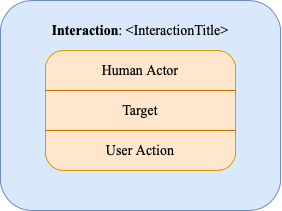
\includegraphics[width=7.5cm]{Figures/Conceptual Model/InteractionBlock.png}
	\caption{Interaction - graphical representation}
	\label{fig:InteractionBlock}
\end{figure}

Some examples of interactions that can be created and customised according to the experience are given below: 
\begin{itemize}
    \item The experience designer can model a "Proximity In" interaction involving the user as a Human Actor, the Walk In action as a User Action and the Virtual Object as an Actuator. 
    \item The experience designed using HMDs allows the user to interact with the Virtual Object by tapping (User Action: Tap) on a 3D Model (Actuator) to "Select the Object" (Effect). A subsequent Tap allows the user the next interaction, for example to play the content. 
\end{itemize}

\subsubsection*{System Event}
The \emph{System Event} provides the signal that triggers the event call. The stimuli generated by the events are, of course, outside the direct control of the user \autoref{fig:SystemEvent}.
\begin{figure}[h]
	\centering
	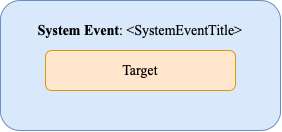
\includegraphics[width=7.5cm]{Figures/Conceptual Model/SystemEvent.png}
	\caption{System Event - graphical representation}
	\label{fig:SystemEvent}
\end{figure}

The System Event is a building block in the same way as the Interaction block, with the difference that neither the Human Actor nor the User Action appears. The only element contained in the System Event block is the Non-Human Actor that participates in the System generated Event.
An example of a System Event is the Beacon Reception. This is a Bluetooth-based technology that allows Bluetooth devices to transmit and receive small messages within short distances. The system is able to recognise the wireless device and the effects triggered can be multiple and show up on one or more Non-Human Actors. 

\subsubsection*{Task}

\emph{Task} is defined as an interaction or system event that generates an effect. \autoref{fig:Task} shows how it embeds two blocks connected by an arrow, recalling a cause-and-effect scenario.
\begin{figure}[h]
	\centering
	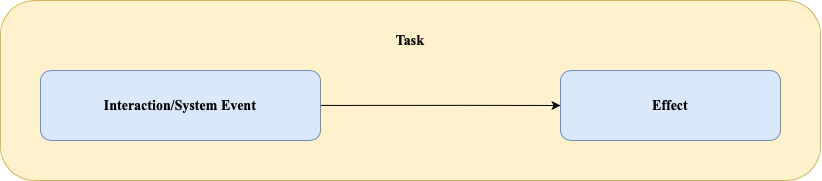
\includegraphics[width=12cm]{Figures/Conceptual Model/Task.png}
	\caption{Task - graphical representation}
	\label{fig:Task}
\end{figure}

The Task can be either user or system dependent. It is described by a sub-model using the building blocks presented so far. 
The user-dependent Task is represented by the presence of the Interaction block, which defines the User Actions that the user can do on one or more Non-Human Actors, combined with the Effects generated on one or more Non-Human Actors. Interactions are seen in detail with respect to the higher level sub-model which will be described later. 
A Task that depends on a System Event defines perceptible Effects on the system and the environment. A change in state of a system device (e.g., "increase in display brightness") is not generated as a response to explicit and intentional human actions in the XR experience, but instead results from phenomena perceived by Non-Human Actors, such as common devices like our smartphones that recognise the decrease in natural light.
At this level, the general purpose of the Task is set out with a representative sentence devised by the experience designer. The composition of the Task should be quite intuitive and straightforward after defining its atomic components individually.
By combining primitives representing an interaction (Human Actor, User Action, Target) or a System Event (Target) it is possible to associate the Effect that is generated on the Actuator. The following table shows an example overview of the many possible combinations. 

\begin{table}[h]
\centering
\begin{tabular}{|c|c|c|c|c|c|}
\hline
\rowcolor[HTML]{DAE8FC} 
\multicolumn{4}{|l|}{\cellcolor[HTML]{DAE8FC}{\color[HTML]{333333} Interaction/System Event}} &
  \multicolumn{2}{l|}{\cellcolor[HTML]{DAE8FC}{\color[HTML]{333333} Effect}} \\ \hline
\rowcolor[HTML]{FFE6CC} 
\multicolumn{1}{|l|}{\cellcolor[HTML]{FFE6CC}\begin{tabular}[c]{@{}l@{}}Human\\ Actor\end{tabular}} &
  \multicolumn{1}{l|}{\cellcolor[HTML]{FFE6CC}\begin{tabular}[c]{@{}l@{}}User\\ Action\end{tabular}} &
  \multicolumn{2}{l|}{\cellcolor[HTML]{FFE6CC}Target} &
  \multicolumn{1}{l|}{\cellcolor[HTML]{DAE8FC}} &
  \multicolumn{1}{l|}{\cellcolor[HTML]{DAE8FC}Actuator} \\ \hline
 &
  \begin{tabular}[c]{@{}c@{}}Press, \\ Click, \\ Speak\end{tabular} &
  Device &
   &
  \begin{tabular}[c]{@{}c@{}}Screenshot Acquisition,\\ Recording Acquisition,\\ Acquired Element saved,\\ Speech to text\end{tabular} &
  Device \\ \cline{2-6} 
 &
  Frame &
   &
  QR Code &
   &
  \begin{tabular}[c]{@{}c@{}}Device, \\ E, VO\end{tabular} \\ \cline{2-2} \cline{4-4} \cline{6-6} 
\multirow{-3}{*}{User U} &
  Frame &
   &
  RFID &
   &
  \begin{tabular}[c]{@{}c@{}}Device,\\ E, VO\end{tabular} \\ \cline{1-2} \cline{4-4} \cline{6-6} 
- &
  - &
  \multirow{-3}{*}{\begin{tabular}[c]{@{}c@{}}Interaction\\ Placholder \\ (IP)\end{tabular}} &
  Beacon &
  \multirow{-3}{*}{Show, Hide} &
  \begin{tabular}[c]{@{}c@{}}Device,\\ E, VO\end{tabular} \\ \hline
\end{tabular}
\caption{ Task Combination - Physical Components (PHC)}
\label{tab:PHCtask}
\end{table}

%% ENVIRONMENT
\begin{table}[h]
\centering
\begin{tabular}{|c|c|c|c|c|}
\hline
\rowcolor[HTML]{DAE8FC} 
\multicolumn{3}{|l|}{\cellcolor[HTML]{DAE8FC}{\color[HTML]{333333} Interaction/System Event}} &
  \multicolumn{2}{l|}{\cellcolor[HTML]{DAE8FC}{\color[HTML]{333333} Effect}} \\ \hline
\rowcolor[HTML]{FFE6CC} 
\multicolumn{1}{|l|}{\cellcolor[HTML]{FFE6CC}\begin{tabular}[c]{@{}l@{}}Human\\ Actor\end{tabular}} &
  \multicolumn{1}{l|}{\cellcolor[HTML]{FFE6CC}\begin{tabular}[c]{@{}l@{}}User\\ Action\end{tabular}} &
  \multicolumn{1}{l|}{\cellcolor[HTML]{FFE6CC}Target} &
  \multicolumn{1}{l|}{\cellcolor[HTML]{DAE8FC}} &
  \multicolumn{1}{l|}{\cellcolor[HTML]{DAE8FC}Actuator} \\ \hline
 &
  Walk In &
   &
  Show, Hide &
   \\ \cline{2-2} \cline{4-4}
 &
  Walk Out &
  \multirow{-2}{*}{\begin{tabular}[c]{@{}c@{}}Augmented\\ Environment\end{tabular}} &
  Show, Hide &
  \multirow{-2}{*}{E, VO} \\ \cline{2-5} 
 &
  Walk In &
   &
  Show, Hide &
   \\ \cline{2-2} \cline{4-4}
 &
  Walk Out &
  \multirow{-2}{*}{\begin{tabular}[c]{@{}c@{}}Virtual\\ Environment\end{tabular}} &
  Show, Hide &
  \multirow{-2}{*}{E, VO} \\ \cline{2-5} 
\multirow{-5}{*}{User U} &
  \multicolumn{1}{l|}{Look Around} &
  \multicolumn{1}{l|}{\begin{tabular}[c]{@{}l@{}}360° Video \\ Environment\end{tabular}} &
  \multicolumn{1}{l|}{Change User View} &
  \multicolumn{1}{l|}{E, VO} \\ \hline
\end{tabular}
\caption{ Task Combination - Environment (E)}
\label{tab:Envtask}
\end{table}

%% VIRTUAL OBJECT - VISUAL OBJECT
\begin{table}[h]
\centering
\begin{tabular}{|c|c|c|c|c|c|c|}
\hline
\rowcolor[HTML]{DAE8FC} 
\multicolumn{5}{|l|}{\cellcolor[HTML]{DAE8FC}{\color[HTML]{333333} Interaction/System Event}} &
  \multicolumn{2}{l|}{\cellcolor[HTML]{DAE8FC}{\color[HTML]{333333} Effect}} \\ \hline
\rowcolor[HTML]{FFE6CC} 
\multicolumn{1}{|l|}{\cellcolor[HTML]{FFE6CC}\begin{tabular}[c]{@{}l@{}}Human\\ Actor\end{tabular}} &
  \multicolumn{1}{l|}{\cellcolor[HTML]{FFE6CC}\begin{tabular}[c]{@{}l@{}}User\\ Action\end{tabular}} &
  \multicolumn{3}{l|}{\cellcolor[HTML]{FFE6CC}Target} &
  \multicolumn{1}{l|}{\cellcolor[HTML]{DAE8FC}} &
  \multicolumn{1}{l|}{\cellcolor[HTML]{DAE8FC}Actuator} \\ \hline
 &
  \begin{tabular}[c]{@{}c@{}}Tap, \\ Press, \\ Click\end{tabular} &
   &
   &
   &
  \begin{tabular}[c]{@{}c@{}}Select\\ Component\end{tabular} &
   \\ \cline{2-2} \cline{6-6}
 &
  \begin{tabular}[c]{@{}c@{}}Gaze In \\ and Dwell\end{tabular} &
   &
   &
   &
   &
   \\ \cline{2-2}
 &
  Walk In &
   &
   &
   &
  \multirow{-2}{*}{Show} &
   \\ \cline{2-2} \cline{6-6}
 &
  Gaze Out &
   &
   &
   &
   &
   \\ \cline{2-2}
 &
  Walk Out &
   &
  \multirow{-5}{*}{} &
  \multirow{-5}{*}{} &
  \multirow{-2}{*}{Hide} &
  \multirow{-5}{*}{E, VO} \\ \cline{2-2} \cline{4-7} 
 &
   &
   &
   &
   &
  \begin{tabular}[c]{@{}c@{}}Change \\ Position\end{tabular} &
   \\ \cline{6-6}
 &
   &
   &
   &
   &
  \begin{tabular}[c]{@{}c@{}}Change\\ Scale Factor\end{tabular} &
   \\ \cline{6-6}
 &
   &
   &
   &
   &
  \begin{tabular}[c]{@{}c@{}}Change\\ Orientation\end{tabular} &
   \\ \cline{6-6}
 &
  \multirow{-4}{*}{Manipulate} &
   &
   &
  \multirow{-4}{*}{} &
  \begin{tabular}[c]{@{}c@{}}Change\\ Texture\end{tabular} &
  \multirow{-4}{*}{VO} \\ \cline{2-2} \cline{5-7} 
 &
   &
   &
   &
  Model &
   &
   \\ \cline{2-2} \cline{5-6}
 &
   &
   &
   &
   &
  \begin{tabular}[c]{@{}c@{}}Change \\ Offset\end{tabular} &
   \\ \cline{6-6}
 &
  \multirow{-2}{*}{Swipe} &
   &
   &
  \multirow{-2}{*}{Text} &
  \begin{tabular}[c]{@{}c@{}}Change\\ Language\end{tabular} &
   \\ \cline{2-2} \cline{5-6}
 &
   &
   &
  \multirow{-8}{*}{\begin{tabular}[c]{@{}c@{}}Static \\ Object\\ (SO)\end{tabular}} &
  Image &
  \begin{tabular}[c]{@{}c@{}}Change\\ Image\end{tabular} &
   \\ \cline{2-2} \cline{4-6}
 &
   &
   &
   &
   &
  Play &
   \\ \cline{6-6}
 &
   &
   &
   &
   &
  Pause &
   \\ \cline{6-6}
 &
   &
   &
   &
  \multirow{-3}{*}{} &
  \begin{tabular}[c]{@{}c@{}}Playback\\ Control\end{tabular} &
   \\ \cline{5-6}
 &
   &
   &
   &
  Model &
   &
   \\ \cline{5-6}
 &
  \multirow{-5}{*}{Swipe} &
   &
  \multirow{-5}{*}{\begin{tabular}[c]{@{}c@{}}Dynamic\\ Object \\ (DO)\end{tabular}} &
  Video &
   &
  \multirow{-9}{*}{VO} \\ \cline{2-2} \cline{4-7} 
\multirow{-19}{*}{User U} &
   &
  \multirow{-19}{*}{\begin{tabular}[c]{@{}c@{}}Visual \\ Object\\ (VO)\end{tabular}} &
  \begin{tabular}[c]{@{}c@{}}Operational\\ Object \\ (OO)\end{tabular} &
   &
  \begin{tabular}[c]{@{}c@{}}Active\\ Custom\\ Action\end{tabular} &
  E, VO \\ \hline
\end{tabular}
\caption{ Task Combination - Virtual Object (VO), Visual Object (VIO)}
\label{tab:VIOTask}
\end{table}

%% VIRTUAL OBJECT - AUDITORY OBJECT
\begin{table}[h]
\centering
\begin{tabular}{|c|c|c|c|c|c|}
\hline
\rowcolor[HTML]{DAE8FC} 
\multicolumn{4}{|l|}{\cellcolor[HTML]{DAE8FC}{\color[HTML]{333333} Interaction/System Event}} &
  \multicolumn{2}{l|}{\cellcolor[HTML]{DAE8FC}{\color[HTML]{333333} Effect}} \\ \hline
\rowcolor[HTML]{FFE6CC} 
\multicolumn{1}{|l|}{\cellcolor[HTML]{FFE6CC}\begin{tabular}[c]{@{}l@{}}Human\\ Actor\end{tabular}} &
  \multicolumn{1}{l|}{\cellcolor[HTML]{FFE6CC}\begin{tabular}[c]{@{}l@{}}User\\ Action\end{tabular}} &
  \multicolumn{2}{l|}{\cellcolor[HTML]{FFE6CC}Target} &
  \multicolumn{1}{l|}{\cellcolor[HTML]{DAE8FC}} &
  \multicolumn{1}{l|}{\cellcolor[HTML]{DAE8FC}Actuator} \\ \hline
 &
  \begin{tabular}[c]{@{}c@{}}Effects on \\ AO correspond\\ to User Actions\\ on other \\ Actors\end{tabular} &
  \begin{tabular}[c]{@{}c@{}}Auditory \\ Object\\ (AO)\end{tabular} &
   &
  \begin{tabular}[c]{@{}c@{}}Play,\\ Pause,\\ Change\\ Language,\\ Playback\\ Control,\\ Audio\\ Control\end{tabular} &
  Device, VO \\ \cline{2-6} 
 &
   &
   &
  \begin{tabular}[c]{@{}c@{}}Background\\ Sound\end{tabular} &
   &
  Device, VO \\ \cline{2-6} 
 &
   &
   &
  \begin{tabular}[c]{@{}c@{}}Object-associated\\ Sound\end{tabular} &
   &
  VO \\ \cline{2-6} 
\multirow{-4}{*}{User U} &
   &
   &
  \begin{tabular}[c]{@{}c@{}}External\\ Source\end{tabular} &
   &
  Device, VO \\ \hline
\end{tabular}
\caption{ Task Combination - Virtual Object (VO), Auditory Object (AO)}
\label{tab:AOTask}
\end{table}

\subsection*{Design of the Activity: High-Level Conceptualization}
The high-level Activity conceptualisation sub-model is defined as a compression of the low-level conceptualisation sub-model. It attempts to organise the individual Tasks and specifically the interactions and related effects, so as to construct a sequence that leads the user to the achievement of a particular end. This model does not go into detail about the individual elements that compose it, but rather aims to design the series of steps that the user must complete in order to reach the goal. 

\subsubsection*{Activity}
The \emph{Activity} is defined as a flow of Tasks. The description of the flow defines the order in which the Tasks must be executed to build the whole experience. Figure \autoref{fig:Activity} represents the Activity as a collector of Tasks, from the starting Task 0, to the N-th Task that marks the conclusion of the single Activity. 
\begin{figure}[h]
	\centering
	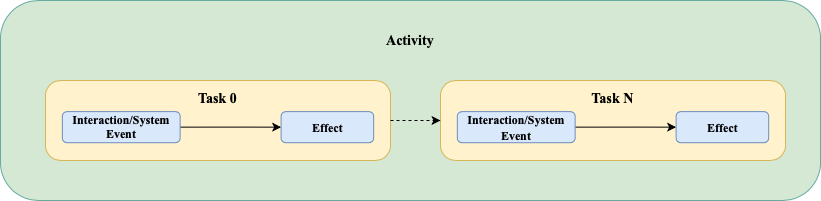
\includegraphics[width=13cm]{Figures/Conceptual Model/Activity.png}
	\caption{Activity: graphical representation}
	\label{fig:Activity}
\end{figure}

To describe the sequence of the actions we decided to use a well-known notation, namely the concepts derived from the BPMN 2.0 model.
The BPMN notation \footnote{http://www.bpmn.org} was developed by the "Business Process Management Initiative" and the "Object Management Group" \footnote{http://www.omg.org}, non-profit associations bringing together operators in the field of information technology and organisational analysis. The BPMN aims to provide an effective representation standard that is easy to use and understand by business users interested in the problem of modelling, design and possible digitalisation of business processes.
The BPMN is essentially a derivation of the formalism of flow charts but with some additions and modifications that make it possible to overcome certain limitations in the modelling of business processes. It makes it possible to construct business process diagrams (BPD) that represent graphs or networks made up of "objects" represented by the process operations, connected by control flows that define the logical relationship, dependencies and order of execution of the operations themselves. 
The BPMN standard defines some basic graphical elements, divided into four categories. We have imported and re-adapted, according to our needs, only two of these categories, considered fundamental to describe the Activities of our model: flow and connecting objects. Flow objects include:
\begin{itemize}
    \item Event: The Event is represented by a circle (\autoref{fig:ActivityElements}) and represents something that happens during a process. Events can have a "cause" that triggers them and a possible "outcome". There are three types of events depending on their location within the flow of a process: start, intermediate and end.
    \item Node: The Node is represented with a blunt rectangle, indicating what we have previously defined as a Task that is carried out within the process considered (\autoref{fig:ActivityElements}). In the official BMPN 2.0 version the Node is called Activity. To avoid ambiguity with the Activity we defined as a flow of Tasks, we chose the term Node. Moreover, a Node represents an elementary and "atomic" entity, i.e. not further decomposable, the BMPN Activity, instead, can also include complex tasks.
    \begin{figure}[h]
	\centering
	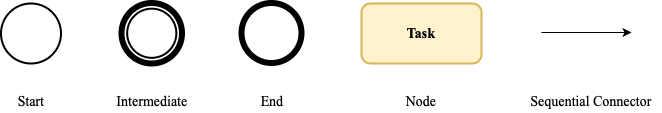
\includegraphics[width=12cm]{Figures/Conceptual Model/ActivityElements.png}
	\caption{Activity Flow Objects - Event, Node and Sequence flow}
	\label{fig:ActivityElements}
    \end{figure}

    \item Gateway: The Gateway is represented by a rhombus (\autoref{fig:Gateways}), it defines the points of the Activity where Task flows diverge or converge. It is used to represent traditional decision points as in classic flow charts, but also simple bifurcations of the Task flow into parallel Tasks or conversely the rejoining of parallel Tasks into a single flow. In other words, Gateways alter the normal direct temporal sequences determined by simple connecting elements, introducing the notion of parallelism, synchronisation and alternative paths. Let us consider the following types of gateway:
    \begin{itemize}
        \item Exclusive: Used to create alternative flows in a Activity. Since only one of the paths can be taken, once a Task has been executed, the others can no longer be executed.
        \item Event-driven: the condition that determines the Task to be executed is based on an evaluated event, a condition on the state of the system to be respected.
        \item Parallel: links several Tasks and indicates that each of them can be executed in parallel without evaluating any condition.
        \item Inclusive: used to create alternative flows in which all tasks are evaluated.
    \end{itemize}
    \begin{figure}[h]
	\centering
	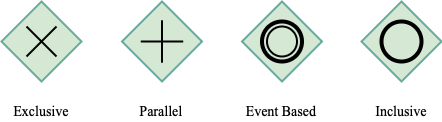
\includegraphics[width=10cm]{Figures/Conceptual Model/Gateways.png}
	\caption{Activity Flow Objects - Gateways}
	\label{fig:Gateways}
    \end{figure}
    
\end{itemize}
In a process the flow elements (events, nodes or gateways) represent "what actually happens" so they must be logically connected to each other. This is what connectors are for. 

\begin{itemize}
    \item Sequence flow: is drawn with a filled arrow \autoref{fig:Activity} and is used to indicate the logical-sequential order between Nodes and Events. 
\end{itemize}
